\documentclass[12pt]{article}
\usepackage[utf8]{inputenc}
\usepackage[margin=1.1in]{geometry}
\usepackage{graphicx}
\usepackage{multicol}
\usepackage{amsmath}
\usepackage[font={small,it}]{caption}

\title{\vspace{-2em}A Statistical Analysis of the Extreme Properties of Solar Wind}
\author{Benedek Kovács\\ Supervisor: Prof. Jim Wild}
\date{} 

\begin{document}
\pagenumbering{roman}
\newgeometry{margin=1.6in}
\maketitle
\begin{center}
        \makebox[\textwidth]{
\includegraphics[width=\textwidth]{fig_other/LU_Logo_Physics.jpg}}
\end{center}
\bigskip
\begin{abstract}
    
\end{abstract}
\newpage
\restoregeometry
\tableofcontents
\newpage
\pagenumbering{arabic}

\section{Introduction}\label{sec:introduction}
    \subsection{Space Weather Effects}\label{sec:spaceweather}
        Geomagnetic storms are causing a larger and larger headache, as humanity becomes more and more reliant on electricity. In the last approximately 30 years, geomagnetic storms caused at least two major and several minor disturbances, both on the surface of Earth and in satellites. During the storm of 1989, the Hydro-Québec power-system experienced a major blackout, with other, mostly North American countries affects by it as well\cite{1989hydroquebec}. In 2003, the 'Halloween Storm' \cite{2003halloweensweden} caused power outages in Sweden and damaged or completely incapacitated several satellites. Recently, in February 2022, a smaller geomagnetic storm impacted several satellites in low-Earth orbit\cite{2022spacex}.\\ \\
        This report aims to study the properties of the solar wind and the Interplanetary Magnetic Field to infer the possibilities and probabilities of the events mentioned above happening again. This can help in forecasting these events and preventing, or at least limiting the damage caused by them. The main outcomes of this report are estimations of the relationships between return levels and return periods for the Interplanetary Magnetic Field, solar wind velocities and solar wind ram pressures in Section \ref{sec:returnperiod}. Further discussion of these topics and their relations to the return periods of an event similar to the Carrington Event or the 2003 Halloween Storms are examined in Section \ref{sec:carrington} and Section \ref{sec:halloween}.
    \subsection{Previous Studies}\label{sec:prevstudies}
        Previous studies often examine the patterns in solar wind data, but most of the time, these studies only investigate the trends and the fairly common data points, not the extremely small/large or the extremely rare data points. Russell's tutorial on solar wind and the Interplanetary Magnetic Field\cite{2001russell} includes several useful graphs and histograms describing solar wind and the IMF. This includes histograms showing the distribution of magnetic field strength at 1 AU distance from the Sun, which can be seen on Figures \ref{fig:russellBX}, \ref{fig:russellBY} and \ref{fig:russellBZ}. These histograms are great at showing the trends and usual data points, but lack depth at showing data points of extremely small or large IMF strength, as they seem to have a minimum and a maximum cut-off.\\
        Using data described in Section \ref{sec:data}, an array of histograms (Figure \ref{fig:hist_imf}) has been created to show the more extreme values as well.\\ \\ 
        \begin{figure}[t!]
            \begin{minipage}{0.48\textwidth}
                \centering
                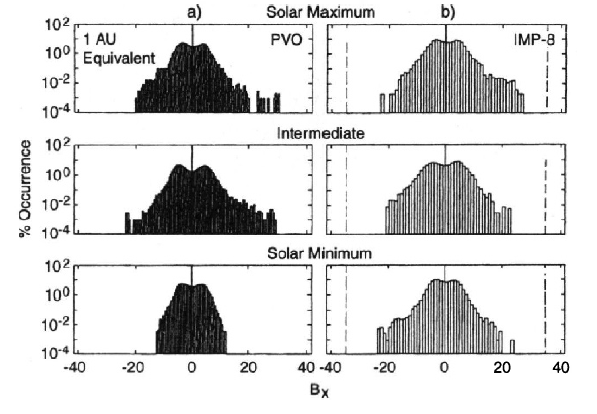
\includegraphics[width=\textwidth]{fig_introduction/russellBX.png}
                \caption{Histograms of the x-component of the Interplanetary Magnetic Field ($B_x$) at a distance of 1 AU from the Sun\cite{2001russell}. The data has been divided into 3 separate batches, based on the solar activity level at the time of measurement. 2 different data sets have been used (PVO 10-minute data on the left and IMP-8 5-minute data on the right).}
                \label{fig:russellBX}
            \end{minipage}
            \hfill
            \begin{minipage}{0.48\textwidth}
                \centering
                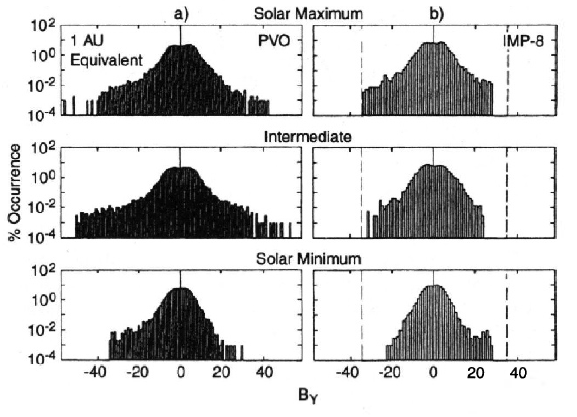
\includegraphics[width=\textwidth]{fig_introduction/russellBY.png}
                \caption{Histograms of the x-component of the Interplanetary Magnetic Field ($B_y$) at a distance of 1 AU from the Sun\cite{2001russell}. The data has been divided into 3 separate batches, based on the solar activity level at the time of measurement. 2 different data sets have been used (PVO 10-minute data on the left and IMP-8 5-minute data on the right).}
                \label{fig:russellBY}
            \end{minipage}
        \end{figure}
        \begin{figure}[t!]
            \centering
            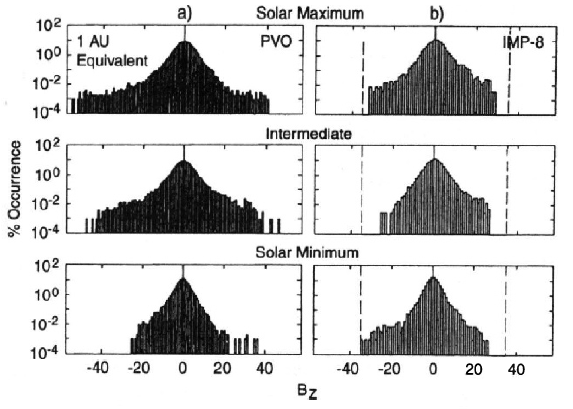
\includegraphics[width=0.48\textwidth]{fig_introduction/russellBZ.png}
            \caption{Histograms of the z-component of the Interplanetary Magnetic Field ($B_x$) at a distance of 1 AU from the Sun\cite{2001russell}. The data has been divided into 3 separate batches, based on the solar activity level at the time of measurement. 2 different data sets have been used (PVO 10-minute data on the left and IMP-8 5-minute data on the right).}
            \label{fig:russellBZ}
        \end{figure}
        \begin{figure}[t!]
            \centering
            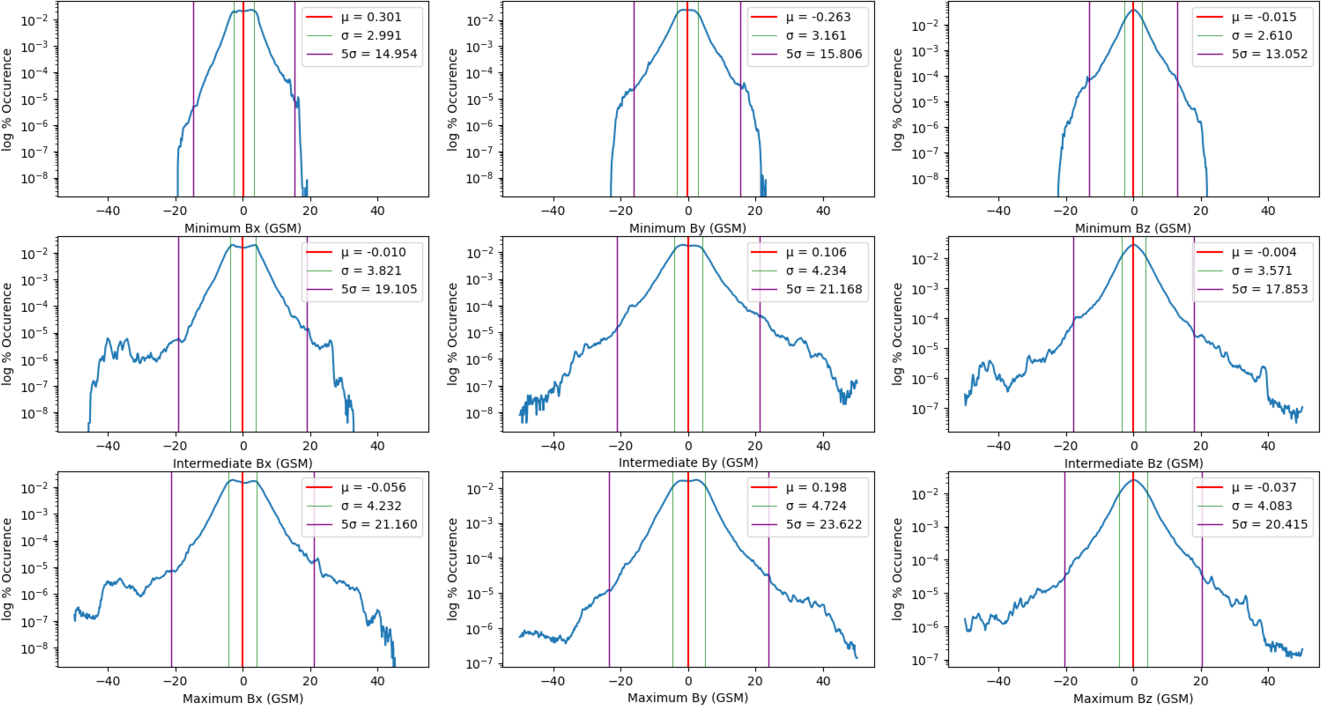
\includegraphics[width=\textwidth]{fig_introduction/hist_imf_strength.png}
            \caption{Histograms showing the strength of the Interplanetary Magnetic Field at Lagrange point L1 (in nT). Data has been separated into 9 different batches based on coordinates in the GSM coordinate system and the solar activity level at the time of measurement. Each row refers to a different solar activity level (minimum, intermediate or maximum) and each column refers to a different coordinate (x, y or z). The red lines indicate the mean, the green lines indicate $1\sigma$ distance from the mean and the purple lines indicate $5\sigma$ distance from the mean.}
            \label{fig:hist_imf}
        \end{figure}
        Comparing Figures \ref{fig:russellBX}, \ref{fig:russellBY} and \ref{fig:russellBZ} to Figure \ref{fig:hist_imf}, 2 important points can be made:
        \begin{itemize}
            \item The middle parts (between approximately $4\sigma -5\sigma$) of the graphs on Figure \ref{fig:hist_imf} almost exactly match the graphs on Figures \ref{fig:russellBX}, \ref{fig:russellBY} and \ref{fig:russellBZ}. This means that even when using slightly different data, anyone could arrive to the same solutions and conclusions.
            \item The end tails on Figure \ref{fig:hist_imf} are not visible on Figures \ref{fig:russellBX}, \ref{fig:russellBY} and \ref{fig:russellBZ}, therefore Figure \ref{fig:hist_imf} is more useful when examining the unusual behaviour of the Interplanetary Magnetic Field outside the zone of influence of Earth's magnetic field.
        \end{itemize}
        It is important to note, that in the following sections, solar wind velocity and magnetic field strength in the x-direction will often be negative. This is due to the fact that the positive x-direction of the GSM coordinate system points from the Earth towards the Sun, therefore solar wind blowing from the Sun will be represented with a negative number, therefore the smaller (more negative) quantities will generally be considered stronger.\\ \\
        Examining Figure \ref{fig:hist_imf}, the quick drop-off at around -20nT on the top row of graphs shows that we can expect no extremely low or extremely high value for magnetic field measurements at the L1 point. More extreme values appear on the graphs of intermediate and maximum solar activity for $B_y$ and $B_z$, but they mostly seem to drop off at a fairly constants rate, suggesting that this is not due to an external effect. This does not seem to hold for the graphs showing the intermediate and maximum solar activity for $B_x$. The end tails in these graphs do not drop off smoothly, but instead have quite a few spikes between -30nT and -40 nT. This suggest that the ordinary behaviour of the IMF breaks, most likely due to an external event, like a coronal mass ejection, which would release a large amount of fast solar wind, carrying a larger magnetic field due to Alfvén's theorem\cite{1976alfven}.
\section{Background Theory}\label{sec:theory}
    \subsection{Properties of Solar Wind}\label{sec:solarwind}
        In 1958, Eugene Parker predicted the existence of solar wind\cite{1958parker}. 8 decades later we understand solar wind a lot better and use modern equipment (e.g. satellites) to measure its properties and the magnetic field brought along with it.\\ \\
        Today, we understand that solar wind is made up of plasma, overwhelmingly made up of electrons and hydrogen nuclei (protons). Solar wind also contains heavier ions in the shape of heavier nuclei (mostly alpha particles), but the overwhelming majority of the solar wind is made up of electrons and protons (approximately 2.5\%-3.6\% of the solar wind consists of helium ions\cite{2006schwenn}). In this report, a composition of 50\% protons and 50\% electrons was assumed. Even though the solar wind is made up of charged particles, on large scales, it is considered neutral, therefore it is called quasi-neutral\cite{2007meyer}. This shows that it is approximately made up of equal number of positively and negatively charged particles.\\
        \begin{table}[t!]
            \begin{center}
                \begin{tabular}{|l|c|c|} \hline
                    &\textit{Slow Solar Wind}&\textit{Fast Solar Wind}\\ \hline
                    Origin&Open magnetic field lines&Coronal holes\\ \hline
                    Speed, $v_p$ ($km\ s^{-1}$)&250-400&400-800\\ \hline
                    Proton Density, $n_p$ ($cm^{-3}$)&10.7&3.0\\ \hline
                    Proton Temperature, $T_p$ ($K$)&$3.4\times 10^4$&$2.3\times 10^5$\\ \hline
                    Electron Temperature, $T_e$ ($K$)&$1.3\times 10^5$&$1\times 10^5$\\ \hline
                    Composition, $n_\alpha /n_p$ ($\%$)&$2.5$&$3.6$\\ \hline
                \end{tabular}
                \caption{A comparison between basic properties of slow and fast solar wind at 1 AU.\cite{2006schwenn} \label{tab:slowfast}}
            \end{center}
        \end{table}\\
        There are two different types of solar wind, which are different from each other to a great extent in their origin and other properties: the slow solar wind and the fast solar wind. Table \ref{tab:slowfast} shows the basic properties of slow and fast solar wind. The most important of these differences are their origin and their their velocity.\\ \\
        Although the exact origins of solar wind is still not understood completely, it is known that slow solar wind originates from open magnetic field lines in the Heliosphere. Due to Alfvén's theorem\cite{1976alfven}, the solar wind plasma flows along magnetic lines (and magnetic field lines follow the flow of plasma), hence it can move away from the Sun along open magnetic field lines. Conversely, fast solar wind originates from coronal holes, which are dense regions of open magnetic field lines. The stronger magnetic field in these regions allows solar wind to escape at a higher rate and higher velocity. Coronal holes are mostly unpredictable and temporary, therefore it is hard to forecast their activity.\\ \\
        The second main difference between slow and fast solar wind is their velocity. The velocity distribution of solar wind in the x-direction is shown in the left-hand side column of Figure \ref{fig:hist_sw}. The variance in the velocity of the slow solar wind is fairly low, between 250km/s and 400km/s. This is most likely due to the reliable and constant nature of its origin. Contrarily, the variance in the velocity of the fast solar wind is fairly high, between 400km/s and 800km/s, although rarely it does flow even faster that (as it is visible on Figure \ref{fig:hist_sw}).\\
        \begin{figure}[t!]
            \centering
            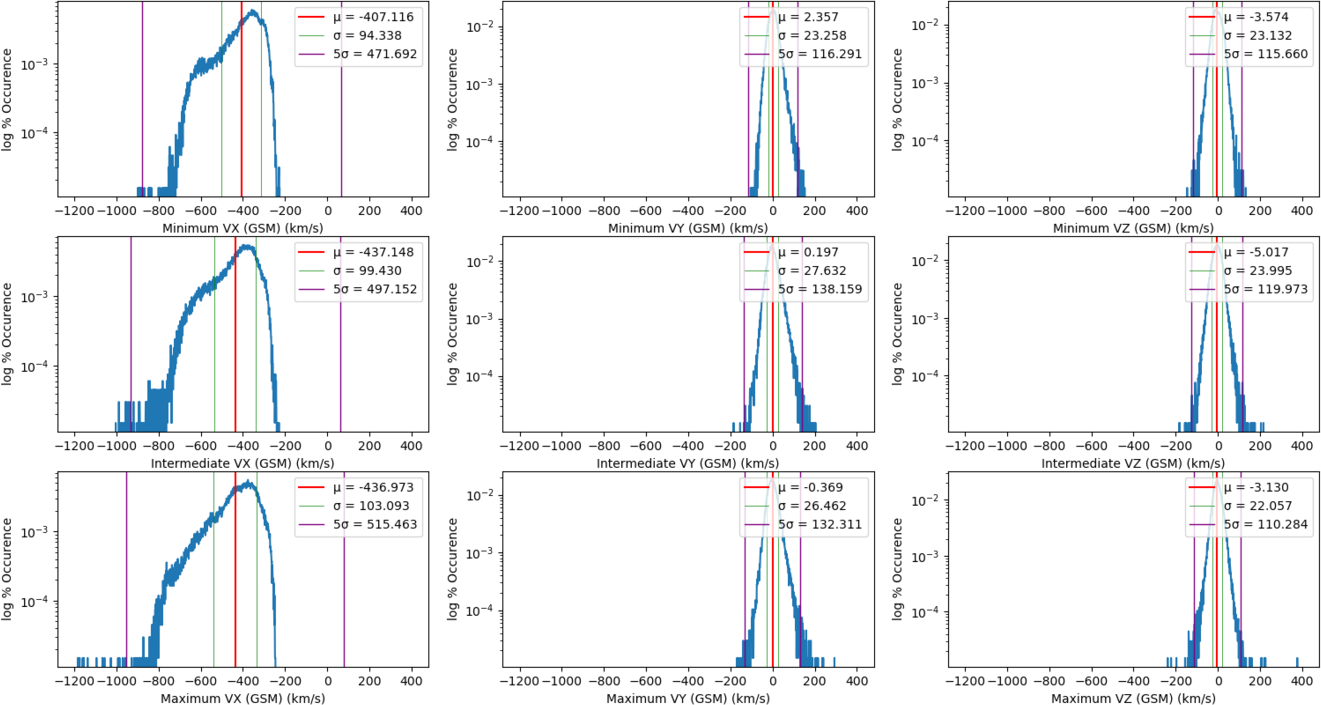
\includegraphics[width=\textwidth]{fig_theory/hist_sw_velocity.png}
            \caption{Histograms showing the velocity of the solar wind at point L1 (in km/s). Data has been separated into 9 different batches based on coordinates in the GSM coordinate system and the solar activity level at the time of measurement. Each row refers to a different solar activity level (minimum, intermediate or maximum) and each column refers to a different coordinate (x, y or z). The red lines indicate the mean, the green lines indicate $1\sigma$ distance from the mean and the purple lines indicate $5\sigma$ distance from the mean.}
            \label{fig:hist_sw}
        \end{figure}\\
        Figure \ref{fig:hist_sw} shows the distribution of solar wind velocity separated based on solar activity level. The most interesting graphs are the histograms of the distribution of $V_x$. $V_y$ and $V_z$ have a fairly even distribution centered around 0km/s with a low variance, no matter the solar activity level. The $B_x$ histograms show a sudden drop at around -250km/s, suggesting that solar wind is rarely slower than that. The most common velocity on these graphs is around -400km/s, which matches the average velocity of slow solar wind\cite{2001russell} (more in Section \ref{sec:solarwind}). A small spike is visible at around -700km/s, which approximately matches the average velocity of fast solar wind\cite{2001russell}. This suggests that slow solar wind is much more abundant, than fast solar wind.
    \subsection{Solar Magnetic Activity Cycle}\label{sec:solarcycle}
        Solar cycles are approximately 11-year long cycles, during which the north pole and the south pole of the Sun switch around. This happens during maximum solar activity (or more accurately, maximum solar activity happens, when the poles of the Sun switch around). The solar activity level (and hence the properties of the cycle itself) are measured by counting the number of sunspots visible on the surface of the Sun. Figure \ref{fig:sunspots} shows the average number of sunspots counted, beginning around 1750. The graphs clearly show a periodicity in the average number of sunspots counted, with a period of approximately 11 years. It is also important to note, that the maximum of every period can extremely differ from each other (e.g. the maximum average sunspot number in Solar Cycle 5 was around 70, while in Solar Cycle 19 it was around 250).\\
        \begin{figure}[t!]
            \centering
            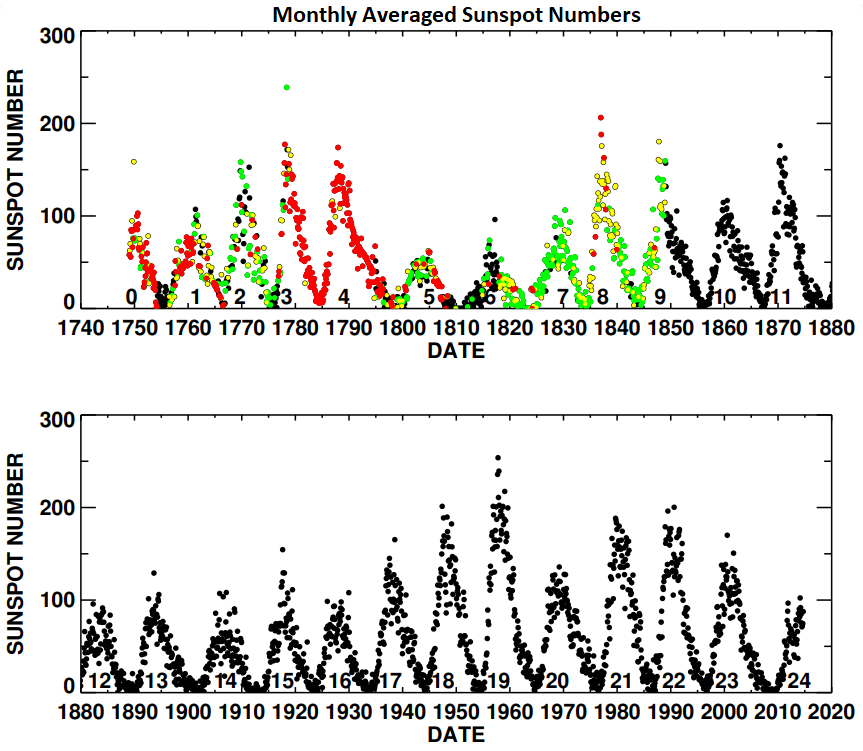
\includegraphics[width=0.8\textwidth]{fig_theory/sunspots.png}
            \caption{The monthly averaged sunspot numbers. Red: more than 20 days of observations missing per month. Yellow: between 11 and 20 days of observations missing per month. Green: between 1 and 10 days of observations missing per month. Black: no observations missing. The numbers above the horizontal axis indicate the number of the solar cycle. An 11-year cycle is clearly visible, as approximately 11 year go by between the spikes. Source: \cite{2015hathaway}}
            \label{fig:sunspots}
        \end{figure}\\
        The solar cycle impacts the number of coronal holes in the corona of the Sun in an unexpected way. Since coronal holes are the primary source of fast solar wind, it is reasonable to assume, that higher solar wind speed measurements are due to more/larger coronal holes. Interestingly, Figure \ref{fig:sw_speeds} show in increase in solar wind speed during the decline to (e.g. 1994) and during the minimum activity periods (e.g. 1986)\cite{2010tokumaru}. This effect is also visible in form of the spike on the top left histogram on Figure \ref{fig:hist_sw}.\\
        \begin{figure}[t!]
            \centering
            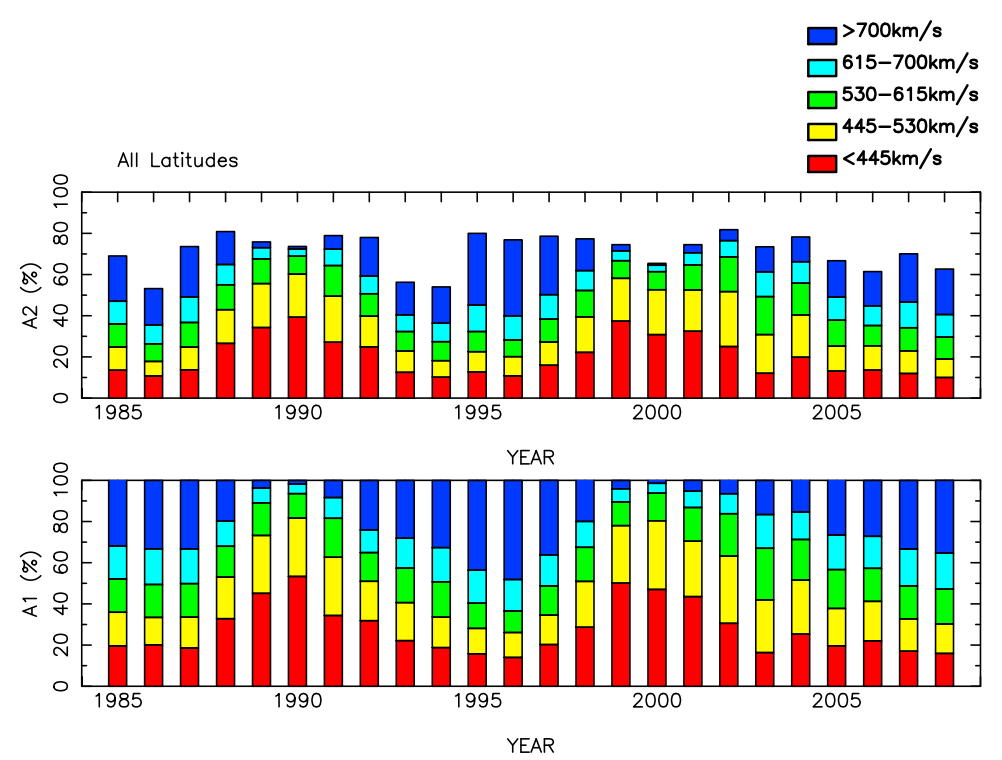
\includegraphics[width=0.8\textwidth]{fig_theory/sw_speed_distribution.PNG}
            \caption{Changes is the fractional areas divided by solar wind speed from 1985 to 2008. On the top, fractional areas compared to the whole surface of the Sun are visible, while on the bottom, fractional areas compared to the measured surface area of the Sun are visible. The colour codes are the following: red: $<445km/s$; yellow $445-530km/s$; green $530-615km/s$; cyan: $615-700km/s$; blue: $>700km/s$. Source: \cite{2010tokumaru}}
            \label{fig:sw_speeds}
        \end{figure}\\
        To observe and understand the different properties of solar wind and the Interplanetary Magnetic Field during different solar activity levels, the data used in this report (more in Section \ref{sec:data}) has been split into 3 categories, based in the solar activity level: minimum solar activity, intermediate solar activity and maximum solar activity. This process required a data set containing the minimum, intermediate and maximum periods, with their start and finish date. For this, data from the SILSO database (\textit{SILSO data/image, Royal Observatory of Belgium, Brussels}) has been used.\\ \\
        The cycles have been split, so that any time period between a minimum and a maximum (and vice versa) have been split into 3 time period with equal length: the third closest to the minimum would be considered to be minimum solar activity, the third closest to the maximum would be considered to be maximum solar activity and the third between these would be considered to be intermediate solar activity. Then, a list of these activity periods was created, including the activity level, the start date and the end date. The method described before means that from 1 full solar cycle, 6 separate activity periods have been created: 2 minimum solar activity periods, 2 intermediate solar activity periods and 2 maximum solar activity periods.
    \subsection{Equipment}\label{sec:equipment}
        The data used in this report has been collected by the MAG and the SWEPAM instruments on the NASA's Advanced Composition Explorer (ACE)\cite{1998ace}. ACE is currently on a close orbit around Lagrange Point 1 (L1). The position of L1 Point and hence the position of ACE is shown on Figure \ref{fig:l1}, marked L1.\\
        \begin{figure}[t!]
            \centering
            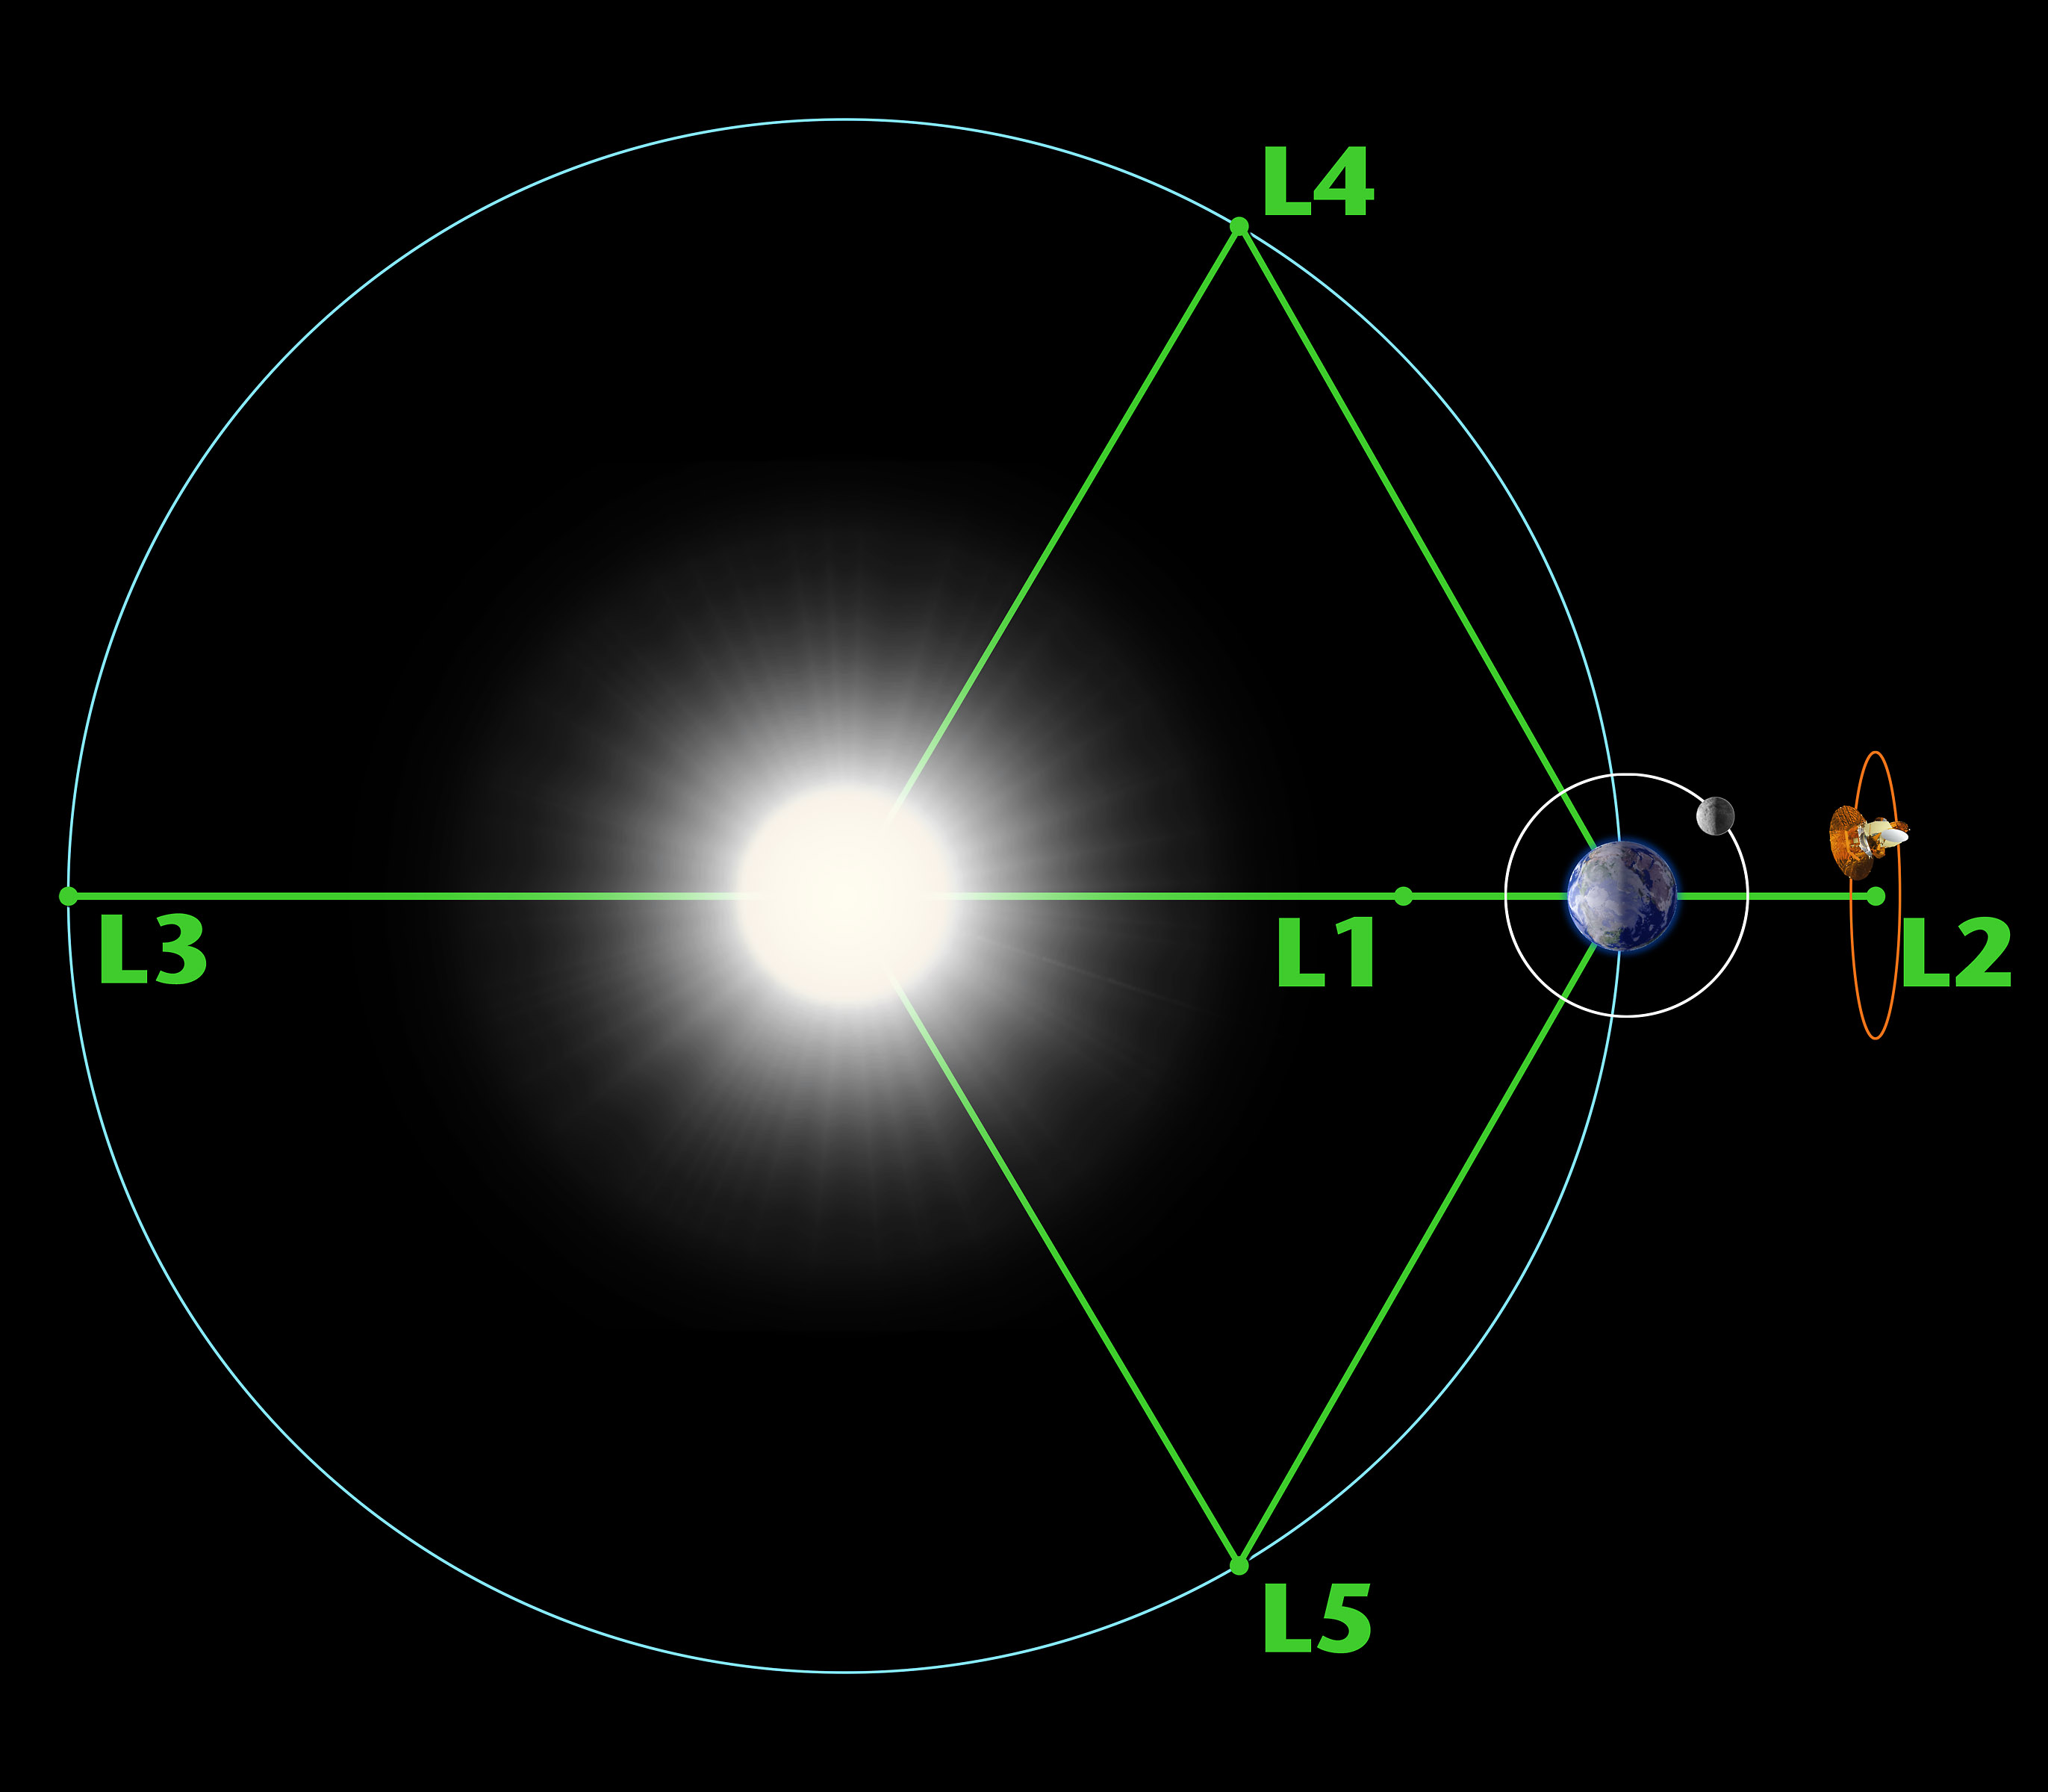
\includegraphics[width=0.6\textwidth]{fig_theory/lagrange.jpg}
            \caption{Positions of Lagrange Points. Lagrange Points are points in space, at which small-mass objects will stay in place, when compared to two certain large-mass objects (e.g. the Sun and the Earth). The ACE can be found orbiting the L1 Point, as it's a great place to measure the properties of the solar wind without having to correct the orbit of the satellite. Source: \cite{lagrangeimage}}
            \label{fig:l1}
        \end{figure}\\
        Measurements of the Interplanetary Magnetic Field have been collected using the magnetometer on the ACE\cite{1998acemag}. Measurements of the solar wind velocity have been collected using the Solar Wind Electron Proton Alpha Monitor on the ACE\cite{1998aceswepam}.
    \subsection{Generalized Extreme Value Distribution}\label{sec:gev}
        The Generalized Extreme Value Distribution is used to model the extreme value of data sets and to extrapolate even more extreme values, using an existing data set. It can model both extremely high or extremely low data, depending on the context. For example modelling extremely high data would be the sea-level in a port. Modelling extremely low data would be the solar wind velocity between the Sun and the Earth, using the GSM coordinate system (due to the coordinate system, the more negative values would be interpreted as more extreme). Multiple different methods and distributions exists to model the extreme values of a data set.\\ \\
        The Generalized Extreme Value Distribution uses the maximum (or minimum) values from several periods of the same length from the same data set (e.g. the maximum value each day). The maximum value from each period is represented by $M_n$:
        \begin{equation}
            M_n = max\{X_1, X_2, ..., X_{n-1}, X_n\}
        \end{equation}
        where $n$ represents the period it's been taken from (e.g. the day the measurement was taken, is one's using daily maxima) and $X_n$ is the nth variable in the given period.\\
        When $n\rightarrow \infty$:
        \begin{equation}
            Pr\Bigg\{ \frac{M_n - b_n}{a_n} \leq z\Bigg\} \rightarrow G(z)
        \end{equation}
        where $G(z)$ is the Generalized Extreme Value Distribution\cite{2001coles}.\\ \\
        The cumulative distribution function for the Generalized Extreme Value Distribution is represented by the following equation\cite{2001coles}:
        \begin{equation}
            G(z) = exp\Bigg [-\Bigg [1+\xi \Bigg (\frac{z-\mu}{\sigma}\Bigg )\Bigg ]^{-1/\xi}\Bigg ]
        \end{equation}
        where $\xi$ is the shape parameter, $\mu$ is the location parameter and $\sigma$ is the scale parameter. If $\xi=0$, the equation above changes to the equation below:
        \begin{equation}
            G(z) = exp\Bigg [exp\Bigg [\Bigg (-\frac{z-\mu}{\sigma}\Bigg )\Bigg ]\Bigg ]
        \end{equation}\\
        Figure \ref{fig:gev} shows the cumulative distribution function and the probability density function of GEV, with varying parameters.\\
        \begin{figure}[t!]
            \centering
            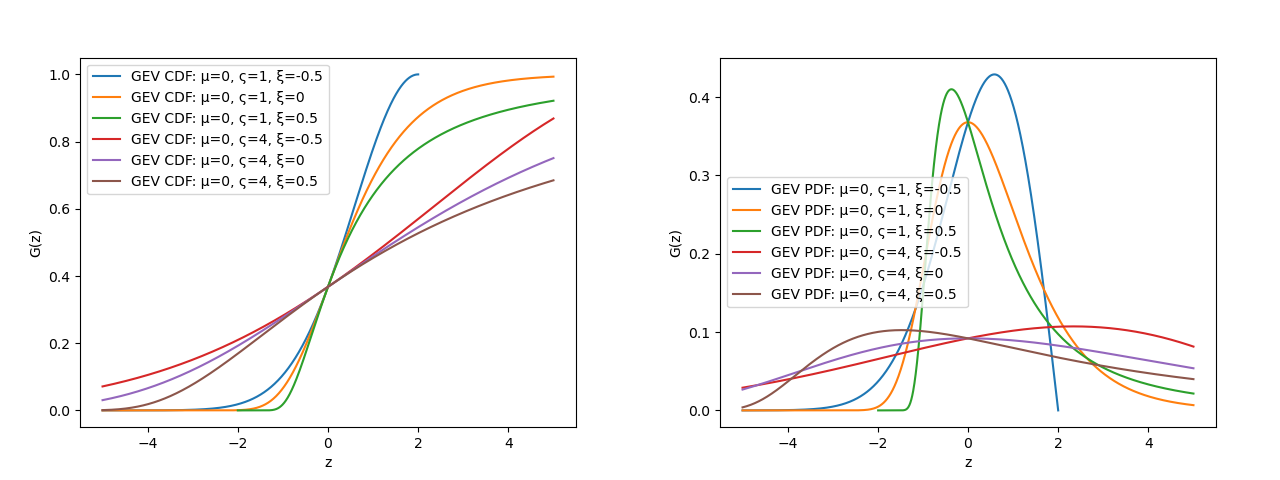
\includegraphics[width=\textwidth]{fig_theory/gev.png}
            \caption{Cumulative distribution functions (left) and probability density functions (right) for the Generalized Extreme Value Distribution, with constant $\mu$ (location) parameter and varying $\sigma$ (scale) and $\xi$ (shape) parameters.}
            \label{fig:gev}
        \end{figure}\\
        To model the distribution of minima, $-z$ should be used instead of $z$. The parameters of the distribution can be determined using several methods (e.g. using maximum likelihood estimation).
    \subsection{Return Levels for Extreme Value Distributions}\label{sec:returnlevel}
        The return level ($z_p$) represents the value expected to be exceeded exactly once during a set period, called the return period ($r$) or conversely, the return period of a value is the period during which the value will be exceeded exactly once.
        The return level can be calculated using the following formula\cite{2001coles}:
        \begin{equation}
            z_p = \mu-\frac{\sigma}{\xi}\Bigg( 1-\Bigg( -ln\Bigg( 1-\frac{1}{r}\Bigg) \Bigg) ^{-\xi}\Bigg)  
        \end{equation}
        where $z_p$ is the return level (or if minima values were used, $-z_p$ is the return level), $\xi$ is the shape parameter, $\mu$ is the location parameter and $\sigma$ is the scale parameter.\\ \\
        To calculate the errors in the return level, one needs to calculate the observed information matrix ($I_E(\xi,\mu,\sigma)$), then use it to calculate the variance-covariance matrix (V):
        \begin{equation}
            I_E(\xi,\mu,\sigma) = 
            \begin{bmatrix}
                    -\frac{\partial ^2l}{\partial \xi^2} & -\frac{\partial ^2l}{\partial \xi \partial \mu} & -\frac{\partial ^2l}{\partial \xi \partial \sigma} \\
                    -\frac{\partial ^2l}{\partial \mu \partial \xi} & -\frac{\partial ^2l}{\partial \mu^2} & -\frac{\partial ^2l}{\partial \mu \partial \sigma} \\
                    -\frac{\partial ^2l}{\partial \sigma \partial \xi} & -\frac{\partial ^2l}{\partial \sigma \partial \mu} & -\frac{\partial ^2l}{\partial \sigma^2}
            \end{bmatrix}
        \end{equation}
        and
        \begin{equation}
            V=I_E^{-1}(\xi,\mu,\sigma)
        \end{equation}
        Using the variance-covariance matrix, the values for the standard error in each parameter can be retrieved, using:
        \begin{equation}
            V=
            \begin{bmatrix}
                    SE_\xi^2 & \ldots & \ldots \\
                    \ldots & SE_\mu^2 & \ldots \\
                    \ldots & \ldots & SE_\sigma^2
            \end{bmatrix}
        \end{equation}
        The variance of the return level then can be calculated using the following formula:
        \begin{equation}
            Var(\hat z_p)\approx \Delta z_p^TV\Delta z_p
        \end{equation}
        where
        \begin{equation}
            \Delta z_p^T=\Bigg [\frac{\partial z_p}{\partial \xi}, \frac{\partial z_p}{\partial \mu}, \frac{\partial z_p}{\partial \sigma}\Bigg ]
        \end{equation}
\section{Method and Data Processing}\label{sec:method}
    \subsection{The Data}\label{sec:data}
        As already mentioned in Section \ref{sec:equipment}, the data used in this report has been collected by the MAG\cite{1998acemag} and the SWEPAM\cite{1998aceswepam} instruments on the NASA's Advanced Composition Explorer (ACE)\cite{1998ace}. The data collected by the MAG instrument (from now on, MAG data), used to analyze the Interplanetary Magnetic Field at L1 ranges from 01/01/1998 to 25/07/2021, while the data collected by the SWEPAM instrument (from now on, SWEPAM data), used to analyze the solar wind speed at L1 ranges from 04/02/1998 to 17/01/2021, meaning that for both data sets, more than 22 years of data has been used. To determine the solar wind ram pressure, data points only found in both of these data sets have been used, therefore the solar wind ram pressure data ranges from 04/02/1998 to 17/01/2021. Both data sets include the data divided in to separate files day by day and include measurements of the strength of the Interplanetary Magnetic Field (MAG data) and the solar wind speed (SWEPAM data) in form of 3-dimensional vectors, representing the data in GSM coordinates. Throughout this report, it should be assumed that data concerning the strength of the Interplanetary Magnetic Field is in units of nT, data concerning the solar wind speed is in units of km/s and data concerning the solar wind ram pressure is in units of nPa.\\ \\
        It is important to note, that while the MAG data includes measurements every second (86400 measurements per day), and hence it can be assumed, that the difference between the measured daily maxima (minima) and the actual daily maxima (minima) is negligible, the same cannot be stated about the SWEPAM data. The SWEPAM data includes measurements every hour (24 per measurements day), therefore a slight difference between the measured daily maxima (minima) and the actual daily maxima (minima) should be expected and the result should be used with caution.\\ \\
        As already mentioned in Section \ref{sec:solarcycle}, data concerning the solar activity periods (more accurately, solar activity maximums and minimums) have been found in the SILSO database (\textit{SILSO data/image, Royal Observatory of Belgium, Brussels}).
    \subsection{Assumptions and Data Processing}\label{sec:dataproc}
        Several assumptions have been made when processing the data and applying distribution functions. These assumptions have been made about the data itself and the behaviour of the solar wind as well:
        \begin{itemize}
            \item It has been assumed, that the data points within each period (from which the maxima and the minima have been selected), the data points would behave like random samples of an arbitrary distribution, and therefore would be independent. This is not entirely true, as the data about the IMF strength and the solar wind speed is driven by several factors, like solar activity, the previous measurements and the state of the IMF (in case of the solar wind speed) or the state of the solar wind (in case of the IMF strength). As solar wind speed and the IMF strength are related due to Alfvén's Theorem\cite{1976alfven}, they depend on each other. In Section \ref{sec:dailydist}, the distributions fitted on the data points show, that this is mostly negligible, due to the large amount of data available.
            \item It has been assumed, that solar wind only consists of electrons and protons. This is relevant, when determining the solar wind ram pressure, as this assumption means heavier ions have not been taken into account when determining the mean mass of solar wind particles. As the abundance of heavier ions in solar wind is small (approximately 5\%\cite{2006schwenn}), this assumption appears to be justifiable.
            \item It has been assumed, that the actual maximum (minimum) value of each day is the largest (smallest) measured value. This assumption has been made due to availability of data.
            \item The solar activity levels have been assumed to have the same time-span from a solar activity minimum to a solar activity maximum (and from a solar activity maximum to a solar activity minimum). This means, that the periods between solar activity minimums and solar activity maximums have been divided to a period of minimum solar activity, intermediate solar activity and maximum solar activity, all of which are the same length. This assumption was made due to a lack of a better method to separate these solar activity levels.
        \end{itemize}\\
        The data processing method to obtain the exact distributions for the Interplanetary Magnetic Field strengths and for the solar wind speeds are almost identical. The method below has been used to produce the distribution graphs in Section \ref{sec:dailydist} (except for the solar wind ram pressure distributions).
        \begin{enumerate}
            \item A list of solar activity periods have been prepared, containing the dates the periods begin and end, and the type of period it is (minimum, intermediate or maximum solar activity).
            \item For every file (one day of measurements), the following process has been followed: the invalid measurements from the IMF strength (and alike from the solar wind speed) data for x, y and z coordinates have been removed and the daily minima and maxima have been determined. These data points have been separated based on coordinate, solar activity the given day belongs to and whether the list contains the minima or the maxima for the given solar activity and coordinate.\label{stepcontinue}
            \item To each of the data points in a list, the ratio of data points lower (higher for minima) has been assigned. For each property (coordinate, solar activity level and minima/maxima), a line of best fit was fitted, using Generalized Extreme Value Distribution and the parameters of the distribution have been determined. Graphs of cumulative distributions functions and probability density functions (based on the parameters determined by the cumulative density functions) have been plotted.
            \item Using the method described in Section \ref{sec:returnlevel}, the errors in the parameters have been determined.
            \item For each property, a graph of return level against return period has been plotted. The return levels have been plotted for return period values between 0.1 year and 1000 years. Then, using the method described in Section \ref{sec:returnlevel}, the errors in the return levels have been determined.
        \end{enumerate}
        The process to plot similar graphs for the solar wind ram pressure includes an additional step. Before determining the maxima and the minima for a period, the following formula has been used to calculate the solar wind ram pressure for every data point in a period:
        \begin{equation}
            P=n*m_p*V^2
        \end{equation}
        where $n$ is the proton density (the electron density is negligible, as electrons have negligible mass and therefore do not contribute to the solar wind ram pressure), $m_p$ is the mass of a proton and $V$ is the solar wind bulk velocity. Then, the daily minima and maxima have been determined and the same process from Step \ref{stepcontinue}. has been followed. It is important to note, that for solar wind ram pressure, the data has not been separated based on coordinates, as solar wind ram pressure in the y and z-directions is negligible.
    \subsection{Distributions of Daily Minima and Maxima}\label{sec:dailydist}
        INCLUDE IMPORTANT GRAPHS AND GENERAL EQUATION FOR CURVES:
        \begin{itemize}
            \item MFI intermediate X minima (show that intermediate activity can cause more extreme effects than maximum activity)
            \item MFI maximum X minima
            \item MFI maximum Z minima (can compare data to Carrington event)
            \item SWE minimum X minima (show that intermediate activity can cause more extreme effects than intermediate and maximum activity)
            \item SWE intermediate X minima (show that intermediate activity can cause more extreme effects than maximum activity)
            \item SWE maximum X minima
            \item pressure intermediate X maxima (show that intermediate activity can cause more extreme effects than maximum activity)
            \item pressure maximum X maxima
        \end{itemize}
    \subsection{Return Levels of Daily Minima and Maxima}\label{sec:returnperiod}
        INCLUDE IMPORTANT GRAPHS AND GENERAL EQUATION FOR CURVES, MAYBE EXACT EQUATIONS FOR EACH GRAPH:
        \begin{itemize}
            \item MFI intermediate X minima (show that intermediate activity can cause more extreme effects than maximum activity)
            \item MFI maximum X minima (maybe just include intermediate or maximum)
            \item MFI maximum Z minima (can compare data to Carrington event)
            \item SWE minimum X minima (show that intermediate activity can cause more extreme effects than maximum activity)
            \item SWE intermediate X minima (show that intermediate activity can cause more extreme effects than maximum activity)
            \item SWE maximum X minima (maybe just include intermediate or maximum)
            \item pressure intermediate X maxima (show that intermediate activity can cause more extreme effects than maximum activity)
            \item pressure maximum X maxima  (maybe just include intermediate or maximum)
        \end{itemize}
\section{Discussion}\label{sec:discussion}
    \subsection{Reaction Time for Measurements at L1 Lagrange Point}
        CALCULATIONS FOR REACTION TIME BETWEEN MEASURING SOLAR WIND AT L1 POINT AND SAID SOLAR WIND HITTING THE SATELLITES AND EARTH
    \subsection{Estimating the Return Period of a 'Carrington Event'-like Geomagnetic Storm}\label{sec:carrington}
        DISCUSS APPROXIMATIONS FOR THE CARRINGTON EVENT. CALCULATE RETURN PERIODS BASED ON BZ AND SOLAR WIND VELOCITY (OR BASED ON ANY OTHER AVAILABLE APPROXIMATIONS, MAYBE MULTIPLE APPROXIMATIONS OF THE SAME QUANTITY). DISCUSS ERRORS IN THE APPROXIMATIONS AND HOW THIS AFFECTS THE RETURN PERIOD.
    \subsection{Estimating the Return Period of a 'Halloween'-like Geomagnetic Storm}\label{sec:halloween}
        DISCUSS MEASUREMENTS FOR THE HALLOWEEN STORM. CALCULATE RETURN PERIODS BASED ON VARIOUS DATA AVAILABLE (MAGNETIC FIELD, SOLAR WIND VELOCITY, RAM PRESSURE). DISCUSS DIFFERENCES IN THESE RESULTS AND HOW THIS AFFECTS THE RETURN PERIOD.
    \subsection{Effects of the Solar Wind on the Magnetopause of Earth}\label{sec:magnetoPAUSE}
        DISCUSS THE DYNAMICS OF MAGNETOSHEATH AND HOW THE RAM PRESSURE AND MAGNETIC PRESSURE BALANCE WORKS. DISCUSS THE RAM PRESSURE (AND HENCE THE SOLAR WIND VELOCITY) NECESSARY TO PUSH THE MAGNETOPAUSE BEHIND THE ORBIT OF GEOSTATIONARY SATELLITES. DISCUSS WHY THIS IS IMPORTANT. DISCUSS RETURN LEVELS FOR THIS SOLAR WIND VELOCITY.
\section{Conclusion/Future Work}\label{sec:conclusions}
    SELF EXPLANATORY, BASED ON THE REST OF THE SECTIONS. CAN EASILY BE CHANGED AFTER THE REST OF THE REPORT HAS BEEN WRITTEN
\newpage
\pagenumbering{alph}

\bibliographystyle{unsrt}
\bibliography{bibliography.bib}

\end{document}